%----------------------------------------------%
% Template Beamer para Apresentações da Asset1 %
%                 %
% Baseado em MIT Beamer Template			   %
% versao 1.1								   %
% Atualizado em 14/12/2021					   %
%----------------------------------------------%
% !TeX spellcheck = pt_BR
\documentclass[t,aspectratio=169]{beamer}
% Para alterar a linguagem do documento
\usepackage[portuges]{babel}
% Para aceitar caracteres especias deretamente do teclado
\usepackage[utf8]{inputenc}
% Para seguir as normas da ABNT de citacao e referencias
\usepackage[alf]{abntex2cite}
% Para incluir figuras
\usepackage{graphicx}
% Para melhor ajuste da posisao das figuras
\usepackage{float}
% Para ajustar as dimensoes do layout da pagina
\usepackage{geometry}
% Para formatar estrutura e informacoes de formulas matematicas
\usepackage{amsmath}
% Para incluir simbolos especiais em formulas matematicas
\usepackage{amssymb}
% Para incluir links nas referencias
\usepackage{url}
% Para incluir paginas de documentos .pdf externos
\usepackage{pgfpages}
% Para ajustar o estilo dos contadores
\usepackage{enumerate}
% Para modificar a cor do texto
\usepackage{color}
% Para incluir condicoes
\usepackage{ifthen}
% Para colocar legendas em algo que nao e float
\usepackage{capt-of}
\usepackage{ulem}

\usepackage{hyperref}
\hypersetup{pdfnewwindow}
\usepackage{fontspec}
\setmainfont[UprightFont={* Regular},BoldFont={* Bold},ItalicFont={* Medium}]{AmpleSoft Pro}

\let\sfdefault\rmdefault

% Para definir o tema do slide
\usetheme{Berlin}
% Para difinir cores e background
\usecolortheme{Asset1}
% Para numerar as figuras
\setbeamertemplate{caption}[numbered]
\beamertemplatenavigationsymbolsempty

%%%%%%%%%%%%%%%%%%%%%%%%%%%%%%%%%%%%
\newcommand{\dt}{202208}
%%%%%%%%%%%%%%%%%%%%%%%%%%%%%%%%%%%%
% Título
\title[Comitê de Risco]{
	Comitê de Risco e Liquidez}

\titlegraphic{
	
\includegraphics[width=0.35\textwidth]{../template/figuras/logoAsset1}
}

% Data
\date{8-setembro-2022}
% Autores
\author[\href{mailto:risco@asset1.com.br}{risco@asset1.com.br}]{
	\href{mailto:mauricio.pereira@asset1.com.br}{Maurício Pereira}\\
	\vspace{0.12cm}
	\href{mailto:matheus.amaral@asset1.com.br}{Matheus Amaral}
}
% Logo do canto inferior direito
\pgfdeclareimage[height=0.45cm]{logoAsset1}{../template/figuras/logoAsset1.pdf}
\logo{
	\vspace*{-0.30cm}
	\pgfuseimage{logoAsset1}
	\hspace*{-0.08cm}}

\AtBeginSection[]{
	\begin{frame}
		\vfill
		\centering
		\begin{beamercolorbox}[sep=8pt,center,shadow=true,rounded=true]{title}
			\usebeamerfont{title}\insertsection\par %\insertsectionhead
		\end{beamercolorbox}
		\vfill
	\end{frame}
}

\begin{document}

%\frame{\titlepage}

{
	\setbeamertemplate{logo}{}
	\begin{frame}
		\maketitle
	\end{frame}
}

%%%%%%%%%%%%%%%%%%%%%%%%%%%%%%%%%%%%%%%%%%%%%%%%%%%%%%%%%%%%%
\section*{Agenda}
\begin{frame}{Agenda}
	\tableofcontents
\end{frame}

%%%%%%%%%%%%%%%%%%%%%%%%%%%%%%%%%%%%%%%%%%%%%%%%%%%%%%%%%%%%%
\section[Pendências]{Pontos Pendentes}
\begin{frame}{Pontos Pendentes}
	\begin{enumerate}
		\item Controle de Risco de Liquidez\\
		Em andamento
		
		\item {\color{blue1}Acompanhamento de IPOs e Follow On}
		
		\item {\color{blue1}Desenvolvimento de Relatório de Risco para o fundo offshore}\\
		Acompanhamento de alertas e restrições do PB
		
		\item {\color{blue1}Revisão e ajustes dos mandatos dos gestores}\\
		Tabela no SQL com os produtos aprovados e verificação automática diária de aderência aos mandatos
		
		\item Adicionar na apresentação o backtest de VaR por Trader.
		
		\item Trazer o acompanhamento de DD rolling 12 months.
		
		\item Adicionar na apresentação a análise de retornos positivos, negativos e acima do CDI por Trader e por produto. 
		
	\end{enumerate}
\end{frame}

%%%%%%%%%%%%%%%%%%%%%%%%%%%%%%%%%%%%%%%%%%%%%%%%%%%%%%%%%%%%%
\section[Resultado]{Atribuição de Resultado}
\begin{frame}{Atribuição de Resultado por \emph{ESTRATÉGIA}}
	\centering
	\includegraphics[width=0.99\textwidth]{figuras/\dt_pnl.pdf}%month_pnl.py
\end{frame}

\begin{frame}{Atribuição de Resultado por \emph{PRODUTO}}
	\centering
	\includegraphics[width=0.99\textwidth]{figuras/\dt_A1 Master FIM_pnl_product.pdf}%pnl_perfattrib.py
\end{frame}

\begin{frame}{Atribuição de Resultado por \emph{Gestor} - Position x Trading}
	\centering
	\includegraphics[width=0.99\textwidth]{figuras/\dt_A1 Master FIM_pnl_trade_position.pdf}%pnl_perfattrib.py
\end{frame}

\begin{frame}{Performance Mensal}
	\centering
	\includegraphics[width=0.99\textwidth]{figuras/\dt_A1 Master FIM_monthBymonth_performance.pdf} %risk_report/fund_performance.py
	\begin{itemize}
		\item \large{Retorno do Master (\%)}\\
		\small{Retorno do CDI (\%)}
	\end{itemize}
\end{frame}

\begin{frame}{Performance e Drawdown}
	\centering
	\includegraphics[width=0.75\textwidth]{figuras/\dt_A1 Master FIM_drawdown.pdf}  %risk_report/fund_drawdown.py
\end{frame}

%%%%%%%%%%%%%%%%%%%%%%%%%%%%%%%%%%%%%%%%%%%%%%%%%%%%%%%%%%%%%
\section[Carteira]{Revisão da Carteira}
\begin{frame}{Correlação entre estratégias}
	\centering
	\includegraphics[width=0.85\textwidth]{figuras/\dt_correl.pdf} 
\end{frame}

\begin{frame}{V@R Backtest} 
	\begin{overlayarea}{\textwidth}{\textheight}
	\begin{columns}[T]
	\column[T]{0.4\linewidth}
	\begin{itemize}
		\item<1->Houve 1 outliers no mês de {\color{blue1} Agosto de 2022}
			\begin{enumerate}
					\item<2->[10-Ago]: VaR 66.5bps \\ PnL {\color{red}-86.1}bps
				\end{enumerate}
			
		\item<3-> Critério de Kupiec na zona de não-rejeição
		\item<4-> Critério de Christoffersen na zona de não-rejeição

	\end{itemize} 
	
	\column[T]{0.6\linewidth}
		\only<1>{
		\includegraphics[width=\linewidth]{figuras/\dt_A1 Master FIM_backtest_1.pdf}%backtest.py
		}	
		\only<2>{
		\includegraphics[width=\linewidth]{figuras/\dt_A1 Master FIM_backtest_2022-08-10.pdf}
		}
		\only<3>{
			\includegraphics[width=\linewidth]{figuras/\dt_A1 Master FIM_backtest_2.pdf}
		}
		\only<4>{
			\includegraphics[width=\linewidth]{figuras/\dt_A1 Master FIM_backtest_3.pdf}
		}

	\end{columns}
\end{overlayarea}
\end{frame}

\begin{frame}{Composição de Risco}
		\centering
	\includegraphics[width=0.99\textwidth]{figuras/\dt_hist_var.pdf} %month_var.py
\end{frame}

%%%%%%%%%%%%%%%%%%%%%%%%%%%%%%%%%%%%%%%%%%%%%%%%%%%%%%%%%%%%%
\section[Limites]{Acompanhamento de Limites}
\begin{frame}{Violações de Limites e Alertas}
	\centering
	\includegraphics[width=0.99\textwidth]{figuras/\dt_trader_var_stress.pdf}%limits.py
\end{frame}

\begin{frame}{Rolagem do mês anterior}
	\centering
	\includegraphics[width=0.77\textwidth]{figuras/\dt_A1 Master FIM_rolagem.pdf}  
\end{frame}

%%%%%%%%%%%%%%%%%%%%%%%%%%%%%%%%%%%%%%%%%%%%%%%%%%%%%%%%%%%%%
\section[Risco]{Controles de Risco e Relatórios}
\begin{frame}{Política de Gestão de Risco de Liquidez - ANBIMA}
	\begin{itemize}
		\item {\color{blue1} Formulação da Política:}\\
		Redação baseada na Política Interna de Risco e exigências da ANBIMA ({\color{green}\checkmark})\\
		\item {\color{blue1} Implementação de Controles:}\\
		Desenvolvimento dos processos complementares descritos na política ({\color{red}X})\\
		\centering
%		\includegraphics[width=0.77\textwidth]{figuras/Looplex - PRV.pdf}
	\end{itemize}
\end{frame}

\begin{frame}{Coeficiente de Diversificação do Fundo}
	\begin{overlayarea}{\textwidth}{\textheight}
		
		\begin{columns}[T]
			\column[T]{0.5\linewidth}
			\centering
			{\color{blue1}\textbf{Fator de Risco}}
			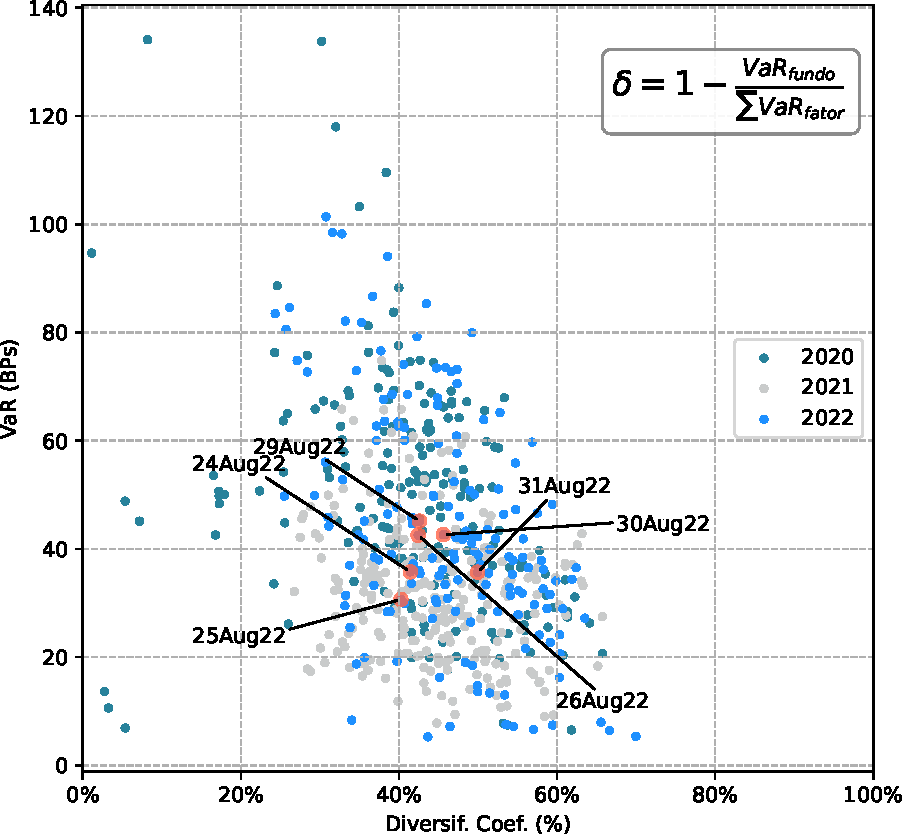
\includegraphics[width=0.9\linewidth]{figuras/202208_diversification.pdf} 
			
			\column[T]{0.5\linewidth}
			\centering
			{\color{blue1}\textbf{Gestor}}
			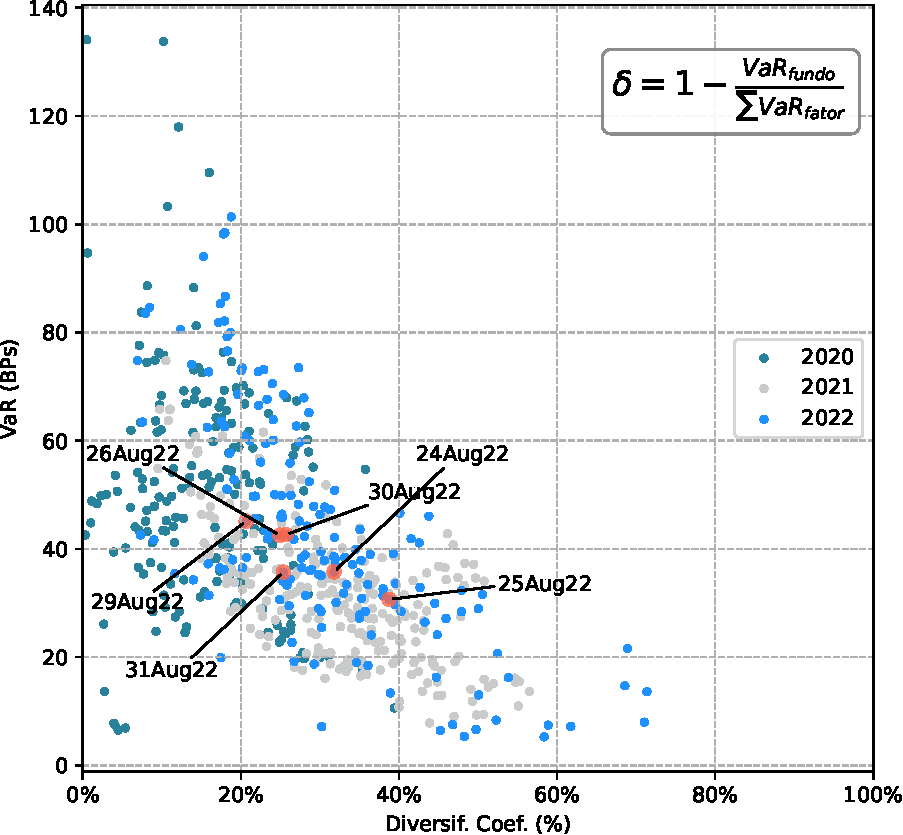
\includegraphics[width=0.9\linewidth]{figuras/202208_diversification_PM.pdf}				
		\end{columns}
	\end{overlayarea}
\end{frame}

%\begin{frame}{Novos limites de Risco por Gestor}
%	{\color{blue1}Risk share:} 
%	\begin{itemize}
%		\item Marcello Siniscalchi: 66.1\%;
%		\item Bruno Carvalho: 41.65\%;
%		\item Pedro Carneiro: 11.90\%;
%		\item Gabriel Blum: 3.57\%;
%		\item Norberto Alves: 3.03\%;
%		\item Marlon Koga: 0.54\%.		
%	\end{itemize}
%	{\color{blue1}Aprovação/revisão de mandatos}	
%	{\color{blue1}Controle utilizando classificação de produtos do Lote45}
%\end{frame}


%%%%%%%%%%%%%%%%%%%%%%%%%%%%%%%%%%%%%%%%%%%%%%%%%%%%%%%%%%%%%
%\section[Outros]{Outros Assuntos Relevantes}
%\begin{frame}{Pontos em aberto}
%	\begin{itemize}
%		\item Trazer tabela de produtos negociados por Trader.
%		\item Apresentar o relatório de Risco e Liquidez atualizado.
%		\item Adicionar na apresentação o backtest de VaR por Trader.
%		\item Trazer o acompanhamento de DD rolling 12 months.
%		\item Adicionar na apresentação a análise de retornos positivos, negativos e acima do CDI por Trader e por produto. 
%	\end{itemize}
		


%\end{frame}

%\begin{frame}{Relatório de Risco do Offshore}
%	\centering
%	\begin{itemize}
%		%\href{file:figuras/offshore_template.pdf}
%		\item Draft \\
%		\centering
%	\includegraphics[width=0.27\textwidth,page=1]{figuras/offshore_template.pdf} 
%		\end{itemize}
%\end{frame}

\end{document}